\section{Subscriptions}

% $Id$

The subscription feature lets you instruct the archive to alert you to new eprints arriving in the archive, by sending you an e-mail at regular intervals.

To create or edit a subscription, click on the ``Subscription'' option on the front page or navigation bar. If you don't have a subscription yet, you'll see a button saying ``Create a subscription.'' It should come as no surprise that this button should be pressed to create a subscription.

Once you have a subscription you should see a form very much like the search form. Use the form exactly how you would a search form. Instead of the ``Search'' and ``Reset the search'' buttons, you'll see the options shown in figure \ref{subscription_options} at the bottom of the form.

\begin{figure}
\centerline{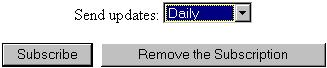
\includegraphics[width=3.2in]{images/subscription-options}}
\caption{\label{subscription_options} Subscription Options}
\end{figure}

The lower two options update your subscription options, and remove the subscription respectively. The popup menu above can be used to determine the frequency with which the system will send you your subscription e-mails. This can be daily, weekly or monthly. You can also set the frequency to ``Never (Off)'',  in case you want to turn off your subscription while you're away without losing all of your subscription criteria.
